\chapter{Travail réalisé}


\section{Aperçu général}
Voici la chronologie du travail réalisé en entreprise.\\

\ganttset{%
	calendar week text={%
		\pgfcalendarmonthshortname{\startmonth}~\startday%
	}%
}
\newganttlinktype{f-m}{
	\ganttsetstartanchor{on right=1}
	\ganttsetendanchor{on left=0}
	\draw[/pgfgantt/link]
	([xshift=-.2pt]\xLeft, \yUpper) --       % xshift to fit arrow
	node[pos=.5, /pgfgantt/link label node] {\ganttlinklabel} 
	(\xRight, \yLower);
}


%vgrid={*1{blue!30},
%	*6{black,dotted},
%	*1{red!30},
%	*2{black,dotted},
%	*1{blue!30},
%	*{34}{black,dotted},
%	*1{green!30},
%	*1{red!30},
%	*{10}{black,dotted},
%	*1{green!30}},
\setganttlinklabel{f-m}{}

\begin{ganttchart}[
	hgrid={*1{black!30,dotted}},
	vgrid={*1{black!30,dotted}},
	x unit=2.91mm,
	time slot format=isodate,
	inline,
	bar/.append style={fill=blue!37},
	bar height=.5,
	group/.append style={draw=black, fill=black!50},
	milestone/.append style={fill=green!20, rounded corners=6pt,scale=2},
	milestone inline label node/.append style={right=1mm},
	]{2019-03-28}{2019-05-25}
	\gantttitlecalendar{year, month=name, week} \\
	\ganttgroup{Analyse des besoins}{2019-03-29}{2019-04-9}\\
	\ganttgroup{Réalisation technique}{2019-04-5}{2019-05-13}\\
	\ganttgroup{Maintenance}{2019-05-13}{2019-05-24} \\
	\ganttbar[bar height=.5]{OFBiz}{2019-04-01}{2019-04-11}\\
	\ganttbar[
	bar/.append style={ fill=red!50
	}]{REST}{2019-04-08}{2019-04-28} \\
	\ganttbar[
	bar/.append style={ fill=orange!50
	}]{Entitymaint}{2019-04-20}{2019-05-12} \\

	\ganttmilestone{Preuve de concept}{2019-05-12}] \\
	\ganttbar[
	bar/.append style={ fill=purple!40, dashed
	}]{Revue de code}{2019-05-13}{2019-05-23} \\
	\ganttlink{elem3}{elem4}
	\ganttlink{elem4}{elem5}
	\ganttlink[link type=f-m]{elem5}{elem6}
	\ganttlink[link type=dr]{elem4}{elem6}
	\ganttlink[link type=f-m]{elem6}{elem7}
\end{ganttchart}

\newpage









\section{Environnement}

\subsection{Installation de l'environnement}
Avant tout, mon intégration a commencé par l'installation du poste de travail suivi par une discussion sur le choix de distribution Linux. Ensuite, la configuration des outils utilisés par l'entreprise ainsi que par la mise en place des accès aux ressources internes. Le choix d'IDE à été fait en faveur de IntelliJ car il possède des nombreux moyens de navigation qui sont incontournables dans la structure de OFBiz riche en dualité XML/Java \ref{dsl}. 




\subsection{Formation générale}


Lors de la formation générale, traditionnellement prévue pour tout les nouveau venus de Néréide, j'ai pu découvrir le fonctionnement basique de OFBiz à travers les démonstration des projets existants. Les points soulevés comportait la gestion des dépendances à travers \verb|Gradle|\footnote{\href{https://gradle.org/}{Moteur de production fonctionnant sur la plateforme Java. }} et \verb|Ant|\footnote{Ant étant déprécié depuis la version 16.11 de OFBiz mais certains projets client l'utilisent toujours car ils se basent sur une version antérieure.  }, une introduction au langage \href{http://groovy-lang.org/}{Groovy} et les raisons pour lesquelles il est préféré au DSL propre à OFBiz \footnote{Pour remplacer le DSL en XML  sous le nom Mini lang, en train d'être entièrement \href{https://cwiki.apache.org/confluence/display/OFBIZ/Mini+Lang+Deprecation}{remplacé}. }


\subsection{Jira}
Un autre point intéressant était le système de gestion de tickets \verb|Jira | utilisé par l'entreprise qui permet de suivre et gérer les bugs tout en interagissant avec les clients. L'outil est utilisé également par la plupart des projets communautaires Apache, dont OFBiz.

\subsection{Approfondissement de Git }
Même si la gestion de versions de OFBiz était historiquement gérée par l'outil Apache \href{https://subversion.apache.org/}{SVN}, dans la gestion de ses propres projets, l'entreprise a fait le choix pour un système plus moderne - \href{https://git-scm.com/}{Git}. 

Alors que j'avais déjà une certaine maîtrise basique de Git, je n'ai jamais eu l'occasion de travailler dans un projet qui comporte des dizaines de branches qui évoluent quotidiennement. Donc, pour monter en compétences sur ce point-là j'ai utilisé le site d'apprentissage conseillé par mon maître de stage: \href{https://learngitbranching.js.org/}{Learn Git Branching}

\subsection{Découverte de communauté libre Apache}
 OFBiz est un projet libre, maintenu par des personnes intéressées qu'on peut catégoriser comme~:
 \begin{labeling}{alligator}
 	\item [\textbf{Contributeurs}] ceux qui suggèrent des modifications utiles aux projets mais ne modifient pas la branche principale.
 	\item [\textbf{Committeurs}] sont des contributeurs responsables de la validation des modifications du framework ainsi que de leur intégration dans le code source du projet. 
 	\item [\textbf{Membres de PMC}] sont responsables des décisions sur la structure générale du projet et sur la cohérence des modifications vis-à-vis de cette dernière  \footnote{PMC acronyme de Project Management Committee (Comité de gestion du projet)}
 \end{labeling}
 
 





\section{Prise en main d'OFBiz}

\subsection{Premier plugin}
Grâce au tutoriel de développement d'une application de base avec OFBiz, j'ai appris à créer mes propres plugins \ref{architecture}. J'ai découvert notamment le mécanisme de définition des entités, ainsi que les moyens de remplissage de la table créée. Ensuite, j'ai défini des nombreux \verb|services| et \verb|events|, d'abord en me basant sur les moteurs par défaut, puis en les définissant moi-même avec Java ou Groovy. Finalement j'ai analysé les techniques qui permettent de visualiser les traitements effectués (front-end).  
\subsection{Projets existants et leur structure}
Tout les projets ont une structure définie dans \ref{architecture}, les projets existant se distinguent notamment par des plugins spécifiques au domaine traité. 

\subsection{Problématique vis-à-vis du développement}
\label{probfonctionnel}
Une majeure partie du développement spécifique consiste à adapter les briques métiers (\emph{application}) combinant des notions de comptabilité, des ressources humaines et les autres aspects qui ne sont pas adaptés à ma formation \footnote{Certaines de ces notions sont enseignées dans le parcours MIAGE.} universitaire. Par conséquent, vu que je ne disposais pas de suffisamment de temps pour les apprendre, j'ai dû me concentrer uniquement sur la partie technique de OFBiz (contenue dans le \emph{framework}).















\newpage


\section{État de l'art}

\subsection{Histoire et problématique des applications web}
Avec l'évolution des technologies du réseau, on a obtenu à la fin des années 60 - début des années 70,  la possibilité d'échanger des informations numériques entre les machines. Cela a permis l'émergence des systèmes d'échanges d'information de plus en plus efficaces. Au début, il s'agissait des architectures très simples, avec une seule couche où une machine unique (\emph{le serveur MainFrame}) effectuait tous les traitements relatifs et qui était accédée par un terminal passif\footnote{Le terme français pour l'équivalent anglais moins gentil, \emph{Dumb terminal} - une machine sans capacité de calcul qui sert uniquement à afficher l'information reçue}. Cela présentait l'avantage d'un système centralisé et homogène facile à implémenter, mais de nombreux inconvénients comme la complexité de maintenance du code monolithique et panne générale en cas d'indisponibilité du MainFrame. \ref{fig:mainframe} 
\begin{figure}[h!]
	\centering
	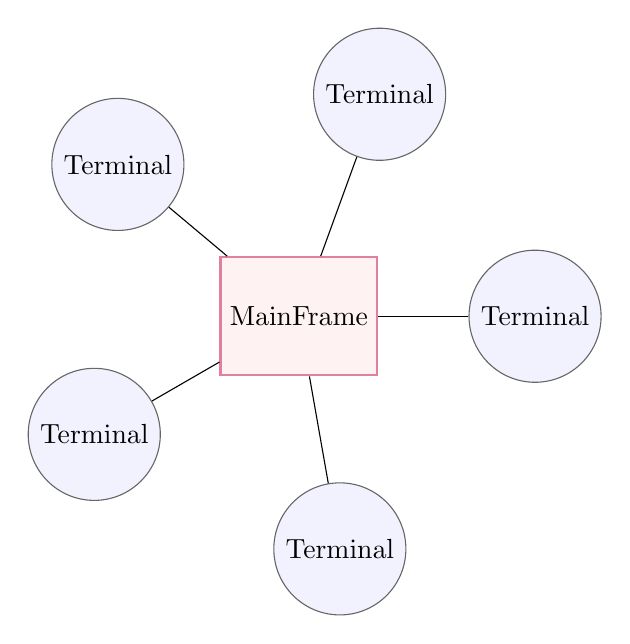
\begin{tikzpicture}
	\def \radius {3cm}
	\node[draw=purple!50,thick,minimum width=1cm,minimum height=1.5cm,fill=red!5] at (300:0mm) (center) {MainFrame};
	\foreach \i  in {0,...,4}{
		\node[draw=black!60, fill=blue!5, circle] at ({\i*70}:\radius) (u\i) {Terminal};
		\draw (center)--(u\i);
	}
	\end{tikzpicture}
\caption{Architecture MainFrame.}
\label{fig:mainframe}
\end{figure}
\\
L'arrivée des ordinateurs personnels a permis la séparation de la couche présentation et parfois aussi  de la couche application qui étaient désormais placés sur la machine des clients. Grâce à cela on a pu proposer des affichages plus sophistiqués (des clients lourds et légers avancés). C'est notamment avec l'arrivée des architectures 2-tiers que la notion de service a été introduite - il s'agit une fonctionnalité fournie par le serveur.


La manière d'invoquer ces services était définie par une interface standardisée, d'où la notion d'API (Application Programming Interface), ou bien interface de programmation applicative qui sert à proposer des points d'entrée pour un nombre de clients de nature différente (utilisateur humain ou une autre machine).
\\ 
Cependant, l'architecture 2-tiers comportait aussi des inconvénients majeurs:
Si le client interagissait avec plusieurs serveurs il devait comprendre l'API de chacun d'entre eux. De plus, c'était dans la responsabilité du client de gérer l'ordre des appels, la cohérence et la combinaison des données reçues. S'ajoutent à cela les serveurs qui pouvaient pas communiquer l'un avec l'autre, résultat - la complexité grandissante des clients. 


L'arrivée d'une architecture à 3 tiers (voire N-tiers avec les couches sécurité, couche routage, etc...) et ainsi que de la notion de Middleware \footnote{Des intergiciels destinés à lier des systèmes informatique de nature différente }  ont apporté un certain nombre d'avantages en matière de réduction de complexité côté client et d'interopérabilité entre ces différentes couches. De plus, de nombreux standards appelées \href{https://fr.wikipedia.org/wiki/Liste_des_sp%C3%A9cifications_des_services_web_WS-*}{WS-*} 
	ont été adoptés afin de combler les failles apparues suite à l'utilisation répandue de Middleware. 
	\begin{figure}[h!]
		\centering
		\begin{tikzpicture}
		[client/.style={circle, draw=red!60, fill=red!5, very thick, minimum size=8mm},
		middleware/.style={rectangle, draw=black!60, fill=black!5, very thick, minimum size=30mm},
		serveur/.style={rectangle, draw=green!90, fill=green!5, very thick, minimum size=8mm}
		]
		%Nodes
		\node[client]      (client)                              {Client};
		\node[middleware]        (middleware)       [right=of client] {Middleware};
		\node[serveur]      (serveur)       [right=of middleware] {Server};
		\node[serveur]      (serveur2)       [above right=of serveur] {Server};
		\node[serveur]      (serveur3)       [below right=of serveur] {Server};
		\node[serveur]      (serveur4)       [above left=of serveur2] {Server};
		\node[serveur]      (serveur5)       [below left=of serveur3] {Server};
		\
		
		\draw[->] (middleware.east) .. controls +(up:7mm) and +(left:20mm) ..   (serveur2.west);
		\draw[->] (client.east) -> (middleware.west);
		\draw[->] (middleware.east) .. controls +(up:10mm) and +(left:5mm) .. (serveur4.west);
		\draw[->] (middleware.east) -> (serveur.west);
		\draw[->] (middleware.east) .. controls +(down:10mm) and +(left:5mm) .. (serveur3.west);
		\draw[->] (middleware.east) .. controls +(down:10mm) and +(left:5mm) ..   (serveur5.west);
		%Lines
		
		\end{tikzpicture}
		\caption{Principe du Middleware.}
		\label{fig:mainframe}
	\end{figure}
	\\
Suite à cela des développeurs et des sociétés ont commencé à mettre en œuvre tout le stack WS-* même pour des tâches où l'utilisation du HTTP suffirait. Concrètement, HTTP était réduit au protocole de transport avec une énorme charge utile XML transmise pour caractériser l'échange. 
\\
Cette approche fonctionne relativement bien dans le contexte d'un seul ou plusieurs organismes qui partagent le même système d'information. Mais dès qu'il s'agit de proposer des services à l'extérieur (à l'échelle mondiale via Internet), cela s'avérait extrêmement compliqué. 
\newpage





\subsection{Representational state transfer}
Dans ce chapitre on va présenter le style architectural REST et comment il répond à des problématiques évoquées dans la section précédente. 
\subsubsection{Histoire}
En 2000, alors que le nombre de sites web dans le monde a atteint 17 millions, Roy Fielding, l'un des contributeurs du standard HTTP et \href{https://tools.ietf.org/html/rfc3986}{URI}, définit REST dans sa thèse de doctorat intitulée \emph{Architectural Styles and the Design of Network-Based Software Architectures} \cite{roythesis}






\subsubsection{Principe}
D'un point de vue abstrait ce style architectural se base sur les technologies fondamentales du World Wide Web: HTTP, Uniform Resource Identifier (URI),  les langages de balisage HTML et XML, ainsi que sur des formats adaptées web comme JSON.\\
REST est un style architectural pour les applications qui interagissent via réseau. Il est défini par six contraintes suivantes: 
\begin{labeling}{rest}
	
\item [\textbf{Uniformité d'interface}] Cette contrainte fondamentale à REST, oblige à manipuler et identifier des ressources uniquement vie leurs représentations(par exemple sous formats HTML, XML ou JSON). Ainsi, chaque représentation fournit suffisamment d'information au client, afin qu'il puisse la modifier ou supprimer.

\item [\textbf{Client-Serveur}] Assure l'absence d'interdépendance entre les clients et les serveurs. Ainsi le serveur propose des services d'une manière générique sans dépendre des spécifications du client (langage de programmation utilisé, plateforme, etc... ). Cela permet au client et au serveur d'évoluer indépendamment. 


\item [\textbf{Sans état}] Les échanges entre le client et le serveur doivent s'effectuer sans conserver l'état de la session sur le serveur entre deux requêtes successives. Le but est d'améliorer les performances du serveur ainsi que l'extensibilité du système. 

\item [\textbf{En couches}] Cette contrainte permet de séparer l'architecture en plusieurs niveaux, cela facilite la passager à l'échelle du système. 
\item [\textbf{Code à la demande}] Ceci est une contrainte facultative qui permet aux serveurs d'étendre ou de modifier le fonctionnement du client grâce à l'envoi du code exécutable.
\item [\textbf{Mise en cache}] Mise en cache de certaines données accédées fréquemment afin d'augmenter les performances. \cite{restcook}

\end{labeling}
 En respectant ces contraintes on a pour objectif de répondre aux mêmes problématiques couverts par les standards WS-* qui sont:
\begin{itemize}
	\item [- \textbf{Séparation des préoccupations}] issu de \emph{l’anglais separation of concerns (SoC)} est le fait de séparer un programme informatique en parties, afin d'isoler des composantes qui répondent à un problème spécifique de la problématique générale.  
	\item [- \textbf{Visibilité}] Comment apprend-on l'existence d'un tel ou tel service? 
	\item [- \textbf{Passage à l'échelle(\emph{scalability})}] Le système sera-t-il capable d'évoluer avec le temps?
	\item [- \textbf{Fiabilité}] Les opérations, ont-elle des effets de bord indésirables? \cite{rest}
\end{itemize}


\subsubsection{En pratique}
Concrètement pour développer une API qui suit les principes REST il faut tout d'abord respecter des règles de nommage des URI. \\
Pour manipuler des ressources, la règle générale est d'utiliser des noms au lieu des verbes.\\
Ainsi, pour récupérer l'ensemble des produits on écrit:
\begin{figure}[h!]
	\begin{lstlisting}[frame=leftline]
example.com/products
	\end{lstlisting}
\end{figure}

au lieu de 


\begin{figure}[h!]
	\begin{lstlisting}[frame=leftline]
example.com/getAllProducts
	\end{lstlisting}
\end{figure}
 
Pour plus de simplicité, on peut diviser les ressources en 4 catégories : \emph{document}, \emph{collection}, \emph{stockage} et \emph{contrôleur}. 

\textbf{Les documents} représentent des objets singuliers qui  correspondent, par exemple, à une entrée en base de données. Il peut être vu comme une ressource dans une ressource de type collection. Pour nommer un document on utilise des noms en singulier : 
\begin{figure}[h!]
	\begin{lstlisting}[frame=leftline]
example.com/api/car-management/managed-cars/{car-id}
example.com/api/client-management/clients/{id}
example.com/api/user-management/users/admin
	\end{lstlisting}
\end{figure}

\textbf{Les collections} sont des dossiers contenant d'autres ressources. Un client peut proposer l'ajout d'une nouvelle ressource pour être rajouté à la collection. C'est à la collection de décider si elle veut accepter la nouvelle ressource ou pas. Ainsi, pour désigner une collection on utilise des noms en pluriel: 
\begin{figure}[h!]
	\begin{lstlisting}[frame=leftline]
example.com/api/car-management/managed-cars
example.com/api/client-management/clients
example.com/api/user-management/users
	\end{lstlisting}
\end{figure}

Quant aux \textbf{stockages}, ce sont des ressources gérées côté client et qui permet de stocker d'autres ressources d'une manière temporaire sans affecter le serveur. Le panier d'achat et la liste des favoris sont des exemples classiques des ressources de stockage: 
\begin{figure}[h!]
	\begin{lstlisting}[frame=leftline]
example.com/api/cart-management/users/{id}/cart
example.com/api/song-management/users/{id}/playlist
	\end{lstlisting}
\end{figure}

Finalement, les \textbf{contrôleurs} servent à exécuter des fonctions, avec les paramètres d'entrée et les valeurs de retour: 
\begin{figure}[h!]
	\begin{lstlisting}[frame=leftline]
example.com/api/cart-management/users/{id}/cart/checkout
example.com/api/song-management/users/{id}/playlist/play-random
	\end{lstlisting}
\end{figure}

\subsubsection{Utilisation des méthodes HTTP}
Les URI ne doivent pas indiquer qu'une opération CRUD est en train d'être effectuée. Les URI doivent seulement identifier la ressource. Au lieu de cela on utilise des méthodes HTTP comme suit: \\
\\
\emph{//retourner tous les utilisateurs\\}
\verb|GET /device-management/user-management/users|\\
\emph{//creer un nouveau utilisateur\\}
\verb|POST example.com/user-management/users|
\\
\\
\emph{//retourne un utilisateur avec cet id\\}
\verb|GET /car-management/users/{id}|\\
\emph{//modifier un utilisateur connu\\}
\verb|PUT /car-management/users/{id}|\\
\emph{//supprimmer un utilisateur connu\\}
\verb|DELETE /car-management/users/{id}|\\



\subsubsection{Examples d'API du style REST}
Afin de voir ce que cela donne en réalité, j'ai décidé d'analyser des services existants qui suivent l'architecture REST. 
L'un des premiers exemples d'API REST traités était celle de \href{https://twitter.com/}{twitter.com}. Ainsi j'ai découvert que twitter permet de concevoir des applications qui interagissent avec le site de manière autonome. 

Par exemple on peut récupérer des statuts des gens en temps réel contenant un certain mot-clé: \\
\verb|GET https://stream.twitter.com/1.1/statuses/filter.json?track=potatoe|\\

Ou bien retourner l'ensemble de messages récents d'un utilisateur donnée:\\
\verb|GET https://api.twitter.com/1.1/statuses/user_timeline.json?user_id=43123|
\\

Un autre exemple intéressant est la navigation du site  \href{https://www.amnesty.org.uk/}{Amnesty International UK}\footnote{ Qui traite des sujets sur les droits de l'homme}:
\\
Ainsi la collection des blogs \\
\verb|www.amnesty.org.uk/blogs/|\\
regroupe des catégories (elles-mêmes des collections): \\
 \emph{Fin de la peine capitale:} \\
 \verb|www.amnesty.org.uk/blogs/anti-death-penalty-project|\\
 \emph{Action étudiante:}\\
 \verb|www.amnesty.org.uk/blogs/student-action-network|\\
 \emph{Réflexion au sujet du traité sur le commerce des armes comme la ressource de la collection "action étudiante":} \\
 \verb|www.amnesty.org.uk/blogs/student-action-network/arms-trade-treaty-last-my-reflections| \\
 et ainsi de suite...
 

\subsection{Implementations existantes}
Finalement, j'ai décidé d'analyser des framworks REST qui permettent de développer des API suivant ce style architectural. Cela avait pour le but soit d'intégrer ce système dans le contexte d'OFBiz.
\subsubsection{Camel}
Apache Camel est un framework libre destiné à faciliter l'intégration des composantes dans le contexte d'entreprise. Il fournit un certain nombre de DSL dont \href{https://camel.apache.org/rest-dsl.html}{Rest DSL} qui est destiné à aider les développeurs à définir les API REST. 
L'un des points particulièrement intéressant de Camel Rest DSL est sa similitude aux techniques utilisées dans l'OFBiz, notamment les DSL sont utilisées avec Java et XML à la fois. 
Malgré ces avantages, la tache d'interrogation de ce framework s'avère trop coûteuse, car elle nécessiterait la réécriture d'une vaste partie relative aux \verb|HTTPServlet| dans l'OFBiz. 
\subsubsection{JAX-RS}
Un autre framework permettant de concevoir des API REST est JAX-RS de Apache \href{http://cxf.apache.org/}{CXF}. La particularité de cet outil est la gestion des URI via les annotations : 
\begin{figure}[h!]
	\begin{lstlisting}[language=Java,frame=leftline]
@Path("/hello/world")
public class Hello {	
	@GET
	@Produces(MediaType.TEXT_PLAIN)
	public String sayPlainTextHello() {
		return "Hello World";
	}
	\end{lstlisting}
\end{figure}\\
Après avoir réussi à intégrer la servlette de JAX-RS dans le framework OFBiz, 
je me suis rendu compte que la technologie risque de ne pas être accepté par la communauté  car elle aussi implique un travail important de réécriture de l'existant. De plus, les annotation ne sont pas dans l'esprit du projet, donc cette idée a été abandonnée. 

\section{Analyse de l'existant}

Lors de la découverte de OFBiz j'ai prêté particulièrement attention à la gestion des échanges web afin d'identitifier les points importants relatifs à l'implémentation des services REST. 


\subsection{Gestion des application web dans OFBiz}


Le groupe des classes d'OFBiz, responsables de la gestion des applications web se basent sur les patrons de conception de   \href{http://www2.sys-con.com/itsg/virtualcd/java/archives/0701/malks/index.html}{"J2EE Presentation Tier"}. Notamment la classe \verb|ContextFilter| qui assure la sécurité des requêtes, implémente le pattern \verb|Decorating Filter|  les vues générées par les moteurs de widgets et les FTL correspondent quand à eux au pattern \verb|Composite View|.
\subsection{ControlServlet}
La classe qui est au cœur du traitement des requêtes, \verb|ControlServlet| correspond au pattern \verb|FrontController|.
Une fois la requête a franchi les filtres de sécurité, la \verb|ControlServlet| initialise l'environnement d'OFBiz, cela inclut les \verb|Entity Delegator|, responsable du modèle de données, ainsi que  \verb|Service Dispatcher| qui exécute les services. Finalement, la session est initialisée et toutes les informations utiles sont stockées dans cette dernière. Une fois l'environnement en place la classe délègue le traitement au \verb|RequestHandler|.

\subsection{RequestHandler}
Cette classe récupère l'ensemble des associations des requêtes(\verb|request-map|) définis sous format XML dans le fichier controller.xml. Il s'agit des associations entre les URI et les vues optionnelles. À part les vues, les URI peuvent être associées à un certain \verb|Event|. Les \verb|events| traitent la logique spécifique, en interagissant avec le moteur des entités ou en appelant un service au travers du moteur correspondant. 
\\
\\
\\
\subsection{Controleur.xml}
La structure des \verb|request-map| est définie comme suit:
\begin{figure}[h!]
	\begin{lstlisting}[language=XML,frame=leftline]
<request-map uri="checkLogin" edit="false">
    <description>Verify a user is logged in.</description>
    <security https="false" auth="false"/>
    <event type="java" path="LoginEvents" invoke="checkLogin"/>
    <response name="success" type="view" value="name" />
    <response name="error" type="view" value="login" />
</request-map>
	\end{lstlisting}
\end{figure}\\
\\
\subsection{API en cours}
Après avoir analysé plusieurs applications web dans OFBiz je me suis rendu compte que le style actuel correspond à celui de \emph{Remote Procedure Call }(RPC), connu pour ses problèmes de performance et du passage à l'échelle. 

\subsection{Mécanisme de résolution des URI}
Les URI de \verb|request-map| ne contiennent pas plus d'un seul mot (d'où RPC) comme par exemple:
\begin{figure}[h!]
	\begin{lstlisting}[frame=leftline]
uri="createEmptyShoppingList"
	\end{lstlisting}
\end{figure}\\
ou bien \\
\begin{figure}[h!]
	\begin{lstlisting}[frame=leftline]
uri="removeFromShoppingList"
	\end{lstlisting}
\end{figure}\\
Ainsi, la résolution d'URI consiste  tout simplement  à vérifier la présence de la clé dans l'objet \verb|Map| contenant l'ensemble des définitions du \verb|controller.xml|.
    


\subsection{\textit{OverrideView()} et le conflit avec les URI segmentées}
Une des spécificités est la gestion des URI segmentés comme dans \\
\begin{figure}[h!]
	\begin{lstlisting}[frame=leftline]
/toto/titi/tata
	\end{lstlisting}
\end{figure}\\
 sont traités par la méthode \emph{String getOverrideViewUri(String path)} qui permet d'appeler une vue sans effectuer de traitement. Le résultat de cela est que toutes les URI segmentées, incontournables à la définition des API du style REST, déclenchent cette méthode qui, à son tour, retourne une erreur. 

\section{Analyse des besoins et attentes de la maîtrise d'ouvrage}
\subsection{Besoins d'évolution}
Avec la popularité du style architectural REST, plusieurs intégrateurs de OFBiz ont montré leur l'intérêt à ce concept. 
Donc afin de répondre aux besoins des utilisateurs et afin d'assurer une meilleure évolutivité des projets basés sur OFBiz à l'avenir, la communauté a lancé une  \href{https://issues.apache.org/jira/browse/OFBIZ-4274}{discussion Jira} où des nombreuses propositions de design ont été faites. 

Après avoir analysé les tentatives et les problématiques d'implémentation de services REST dans OFBiz je suis arrivé à la conclusion qu'une solution de bas niveau répondrait au mieux aux besoins des intéressés. De plus il était évident que la solution doit être développé en parallèle du système actuel, c'est-à-dire sans provoquer de dysfonctionnement au niveau de l'existant.




\section{Réalisations techniques}
\subsection{Choix vers URITemplate}
Même si après l'analyse de la bibliothèque \href{http://cxf.apache.org/docs/jax-rs.html}{JAX-RS de CXF}, j'ai pris la décision de ne pas poursuivre ce chemin, certaines classes m'ont permis de trouver une inspiration en terme de concept qui peut être utilisé dans OFBiz. Ainsi, la classe \href{https://cxf.apache.org/javadoc/latest/org/apache/cxf/jaxrs/model/URITemplate.html}{URITemplate}  permet de créer des modèles de URI avec les variables. \\
Exemple 1: 
Supposons le modèle de URI suivant:
\begin{figure}[h!]
	\begin{lstlisting}[frame=leftline]
/foo/bar/{baz}/{qux}
	\end{lstlisting}
\end{figure}
\\Est mis en correspondance à travers la méthode \emph{.match()} avec l'URI suivant:
\begin{figure}[h!]
	\begin{lstlisting}[frame=leftline]
/foo/bar/toto/titi
	\end{lstlisting}
\end{figure}\\
Par conséquent, notre modèle contient désormais deux entrées de variables avec les clés \verb|[baz, qux]| qui correspondent aux valeurs \verb|[toto, titi]| respectivement. 

Un autre point à noter est la possibilité d'avoir des variables adaptables au moyen d'une expression régulière. Ainsi le modèle 
\begin{figure}[h!]
	\begin{lstlisting}[frame=leftline]
/foo/{v1:\\d}/{v2} 
	\end{lstlisting}
\end{figure}\\
peut être mis en correspondance uniquement avec les URI qui ont un chiffre\footnote{La lettre "d" signifie le mot l'anglais \emph{digit} - "chiffre" en français} en premier argument \verb|v1|.
\subsection{Bibliothèque CXF}
Donc, vu la flexibilité de \verb|URITemplate|, j'ai décidé de l'utiliser au sein d'OFBiz.
Naturellement, l'ajout des dépendances dans un vaste projet comme OFBiz doit être fait avec précaution. La raison: des libraires deviennent souvent dépréciées ou changent à tel point que cela provoque la nécessité de réécrire des parties importantes du projet.  

Après l'analyse des dépendances de OFBiz, j'ai remarqué la présence  de l'outil \href{https://tika.apache.org/}{Apache Tika} qui est utilisé dans le OFBiz pour produire et analyser des fichiers du type XLS ou PDF. Ainsi, Tika contient la bibliothèque CXF ce qui m'a donné la liberté d'utiliser cette dernière. 

\subsection{Intégration en parallèle avec le système existant}
Finalement, j'ai intégré ce système de résolution des URI basé sur la classe \verb|URITemplate| dans le \verb|RequestHandler| de OFBiz. Cela était fait en modifiant légèrement le mécanisme existant. Concrètement, au début de la résolution d'une URI, l'ensemble des \verb|request-map| est délégué au nouveau mécanisme qui, en cas de succès\footnote{ Ayant validé l'URI de la requête avec via la méthode \emph{.match()} avec l'une des modèles construits à partir de l'ensemble de  "request-map"} redirige soit vers la vue, soit vers le \verb|Event| correspondant, indiqués dans la définition de \verb|request-map|. En cas d'absence de "match" via \verb|URITemplate|, la suite de la méthode exécute des traitement de manière traditionnelle.  


\subsection{Nouveau controller.xml}
Grâce à ces modifications, nous avons la possibilité de définir des points d'entrée d'une manière plus flexible:
\begin{figure}[h!]
	\begin{lstlisting}[frame=leftline]
<request-map uri="products/pets/{product-id:\\d}" method="PUT">
...
   <response name="success" type="view" value="viewProduct"/>
...
</request-map>
	\end{lstlisting}
\end{figure}\\
Qui permet de modifier d'un produit animalier identifié un son \emph{product-id} numérique, en appelant la méthode \verb|HTTP PUT|, par exemple. 
\newpage
\subsubsection{Les collisions d'URI}
Cependant, suite à l'introduction du nouveau système, on a rencontré une difficulté mineure quant à la définition des modèles avec les variables.\\
Par exemple lors de la définition de plusieurs \verb|request-map| successives dans un même controller.xml comme suit: \\
\\
\emph{//afficher un stock identifié par la valeur de sa clé primaire}
\begin{figure}[h!]
	\begin{lstlisting}[frame=leftline,language=xml]
<request-map uri="stock/{primary-key-id}" 
\end{lstlisting}
\end{figure}\\   
\emph{//retourner le formulaire de modification d'un stock}
\begin{figure}[h!]
	\begin{lstlisting}[frame=leftline,language=xml]
<request-map uri="stock/form" 
	\end{lstlisting}
\end{figure}\\
\emph{//afficher les relations entre les stock}
\begin{figure}[h!]
	\begin{lstlisting}[frame=leftline,language=xml]
<request-map uri="stock/relations" >
	\end{lstlisting}
\end{figure}  \\
Cette situation suppose que dans la première \verb|request-map| il est impossible d'avoir des clés primaires avec la valeur \verb|"form"| ou \verb|"relations"|. La solution pour ce genre d'exception \footnote{Qui doivent a priori être relativement rares} est l'exclusion des mots spécifiques via des expressions régulières: 
 \begin{figure}[h!]
 	\begin{lstlisting}[frame=leftline,language=xml,frameround=tttt]
... uri="stock/{primary-key-id:(?!(form)|(relations)).*}" 
 	\end{lstlisting}
 \end{figure}  \\


\subsubsection{Testes Mockito}
Finalement, un point intéressant était l'écriture des testes unitaires en utilisant la bibliothèque \href{https://site.mockito.org/}{Mockito}. Des principes et des bonnes pratiques de ces tests m'ont été montrés par mon tuteur de stage. 
\subsection{Modification de la partie "Administration: gestion des entités"  (entitymaint)  }
Afin de montrer l'utilité du nouveau système, j'ai décidé de modifier une partie front existante ainsi que les points d'entrée avec lesquelles elle interagissait.
\subsubsection{Choix de la partie illustrative}
Pour pouvoir tester toute la puissance des méthodes classiques du protocole \verb|HTTP| j'ai dû choisir une partie qui permettait d'effectuer l'ensemble des opérations CRUD. Par conséquent, le choix était porté sur la partie d'administration d'OFBiz qui correspond à la gestion des entités : \verb|entitymaint|.
\subsubsection{Difficultés de modification} 
Vu qu'OFBiz a été construit sans tenir compte de REST, ce genre de modifications impliquent des changements profonds de la structure du code, allant jusqu'à la réécriture complète. Donc, disposant d'un temps limité, j'ai dû avoir recours aux certains compromis comme utilisation d'un même formulaire pour la création et la modification d'une entité.
\subsubsection{Clés composées}
Un autre compromis mineur qui devait être fait, était la présence d'un nombre variable des clés primaires qui identifie une entité-ressource. Par conséquent, la variable qui correspond à l'ensemble des valeurs des clés primaires doit pouvoir accepter un nombre quelconque des clés. Pour cela, on utilise une expression régulière: 

\begin{figure}[h!]
	\begin{lstlisting}[frame=leftline,language=xml,frameround=tttt]
<request-map uri="entity/{entityName}/{pkValues: .*}" method="get">
...
<request-map uri="entity/{entityName}/{pkValues: .*}" method="delete">
...

	\end{lstlisting}
\end{figure}  
\subsection{Stateless}
Un des concepts fondamentaux de REST est l'absence de stockage de l'état côté serveur. 
\subsubsection{Les réalisation par la communauté}
OFBiz, n'étant pas \emph{stateless}\footnote{Sans état - sans conserver des informations} il utilise la session comme un moyen d'authentifier les utilisateurs. Ainsi, les tentatives de supprimer la notion d'état ont été faites par la communauté. Malheureusement, des nombreux concepts se basent sur la  session et la suppression serait trop coûteuse. Au lieu de la supprimer, la communauté à \href{https://issues.apache.org/jira/browse/OFBIZ-9833}{implémenté} l'authentification en utilisant les \href{https://jwt.io/introduction/}{JSON Web Tokens}, mais derrière, la session est toujours utilisée.
\subsection{Divers}
\subsubsection{REST dans un projet client}
Les nouvelles fonctionnalités en matière de définition des API ont été adoptées dans une partie fonctionnelle du projet \emph{Dejbox} \ref{dejbox}. Cela a également entraîné la correction de quelques fonctionnalités du framework. Notamment, l'association d'un code de retour \verb|HTTP| à une réponse spécifique d'un service OFBiz et l'adaptation de l'outil de transformation des objets en JSON.

\subsubsection{Généralisation de code}
Parmi les tâches qui m'ont été confiées, il y avait la généralisation du code spécifique au projet client, afin qu'il puisse être remonté vers la communauté Apache. Il s'agit d'un client qui "consommait" des services du type REST à partir d'une API extérieure. Le but était de rendre le client suffisamment générique pour qu'il puisse prendre en compte les spécificités d'interaction entre les API d'une nature différente (type d'authentification, réponse).


